\documentclass[11pt,a4paper]{article}

% Packages
\usepackage[utf8]{inputenc}
\usepackage[T1]{fontenc}
\usepackage{amsmath,amssymb,amsthm}
\usepackage{mathtools}
\usepackage{bm}
\usepackage{graphicx}
\usepackage[margin=1in]{geometry}
\usepackage{booktabs}
\usepackage{array}
\usepackage{longtable}
% enumitem removed - using standard lists
\usepackage{hyperref}
% cleveref removed
\usepackage{fancyhdr}
\usepackage{xcolor}
% tcolorbox removed - using simple box
\usepackage{caption}
\usepackage{subcaption}
\usepackage{natbib}
\usepackage{tikz}
\usetikzlibrary{arrows.meta,positioning,shapes.geometric}

% Theorem environments
\theoremstyle{definition}
\newtheorem{definition}{Definition}[section]
\newtheorem{proposition}{Proposition}[section]
\newtheorem{lemma}{Lemma}[section]
\newtheorem{theorem}{Theorem}[section]
\newtheorem{corollary}{Corollary}[section]
\newtheorem{remark}{Remark}[section]
\newtheorem{axiom}{Axiom}[section]

% Custom commands
\newcommand{\R}{\mathbb{R}}
\newcommand{\E}{\mathbb{E}}
\newcommand{\Var}{\mathrm{Var}}
\newcommand{\Cov}{\mathrm{Cov}}
\newcommand{\Hstat}{\mathcal{H}_{\text{stat}}}
\newcommand{\Hml}{\mathcal{H}_{\text{ML}}}
\newcommand{\Ocomp}{\mathcal{O}_{\text{comp}}}
\newcommand{\Osens}{\mathcal{O}_{\text{sens}}}
\newcommand{\Osurr}{\mathcal{O}_{\text{surr}}}
\newcommand{\IML}{\mathcal{I}_{\text{ML}}}
\newcommand{\Dcausal}{\Delta_{\text{causal}}}
\newcommand{\Interp}{\mathcal{I}}
\newcommand{\Complex}{\mathcal{C}}
\newcommand{\Manifold}{\mathcal{M}}
\newcommand{\Neigh}{\mathcal{N}}

% Colors
\definecolor{kdenseblue}{RGB}{0,102,204}
\definecolor{statgreen}{RGB}{34,139,34}
\definecolor{mlorange}{RGB}{255,140,0}

% Header/Footer
\pagestyle{fancy}
\fancyhf{}
\fancyhead[L]{\textit{The Formalism of Interpretability Manifolds}}
\fancyhead[R]{\textit{K-Dense Web}}
\fancyfoot[C]{\thepage}
\fancyfoot[R]{\footnotesize Generated using K-Dense Web (\href{https://k-dense.ai}{k-dense.ai})}
\renewcommand{\headrulewidth}{0.4pt}
\renewcommand{\footrulewidth}{0.4pt}

% Title
\title{\textbf{The Formalism of Interpretability Manifolds}\\[0.5em]
\large A Symbolic Mathematical Framework for the Epistemology of\\Interpretable Machine Learning}
\author{K-Dense Web\\
\texttt{contact@k-dense.ai}}
\date{February 4, 2026}

\begin{document}

\maketitle

\begin{abstract}
We present a rigorous mathematical framework for interpretable machine learning (IML), formalizing the field's epistemological structure through the \textit{Interpretability System} tuple $\IML = \langle \mathcal{H}, \mathcal{O}, \mathcal{M}, \Delta \rangle$. Drawing exclusively from the theoretical foundations established in the literature on the evolution of IML, we derive: (1) the \textit{Evolutionary Divergence} between statistical and machine learning regimes characterized by an opacity phase transition; (2) a taxonomy of interpretation operators $\{\Ocomp, \Osens, \Osurr\}$ with formal conditions for applicability; (3) topological violations arising from extrapolation artifacts and uncertainty quantification gaps; and (4) the fundamental causal-predictive divergence. We synthesize these components into an \textit{Interpretation Lagrangian} $\mathcal{L} = \Dcausal + \lambda \Complex(f)$ that captures the irreducible tension between predictive utility and causal fidelity. This formalism provides a unified mathematical language for analyzing the epistemological limits of model interpretation.
\end{abstract}

\vspace{1em}

% Graphical Abstract
\begin{figure}[ht]
\centering

\includegraphics[width=0.85\textwidth]{../figures/graphical_abstract.png}
\caption{\textbf{Graphical Abstract.} The Interpretability System $\IML = \langle \mathcal{H}, \mathcal{O}, \mathcal{M}, \Delta \rangle$ representing the four fundamental components: Hypothesis Space $\mathcal{H}$ (manifold structure), Interpretation Operators $\mathcal{O}$ (Component, Sensitivity, Surrogate), Method Taxonomy $\mathcal{M}$, and Error Metric $\Delta$ (causal divergence measure).}
\label{fig:graphical_abstract}
\end{figure}

\newpage

%==============================================================================
\section{Legend of Variables}
%==============================================================================

\noindent\fbox{\parbox{\textwidth-2\fboxsep-2\fboxrule}{%
\textbf{Symbol Definitions}\\[0.5em]
\begin{longtable}{@{}p{2.5cm}p{10cm}@{}}
\toprule
\textbf{Symbol} & \textbf{Definition} \\
\midrule
\endhead
$\IML$ & Interpretability System tuple $\langle \mathcal{H}, \mathcal{O}, \mathcal{M}, \Delta \rangle$ \\
$\mathcal{H}$ & Hypothesis space (set of all admissible models) \\
$\Hstat$ & Statistical hypothesis space: distributional assumptions, low complexity \\
$\Hml$ & Machine learning hypothesis space: hyperparameter-optimized, opaque \\
$\mathcal{O}$ & Set of interpretation operators $\{\Ocomp, \Osens, \Osurr\}$ \\
$\Ocomp$ & Component operator: extracts structural parameters $\theta$ \\
$\Osens$ & Sensitivity operator: perturbation-based analysis \\
$\Osurr$ & Surrogate operator: local interpretable approximation \\
$\mathcal{M}$ & Method taxonomy (categorical structure of IML methods) \\
$\Delta$ & Error/challenge metric space \\
$\Dcausal$ & Causal divergence: $|f_{\text{pred}} - f_{\text{cause}}|$ \\
$f: \mathcal{X} \to \mathcal{Y}$ & Model function mapping inputs to outputs \\
$\theta \in \Theta$ & Model parameters in parameter space $\Theta$ \\
$\Complex(f)$ & Complexity functional of model $f$ \\
$\Interp(f)$ & Interpretability measure of model $f$ \\
$P(\cdot)$ & Probability measure \\
$\mathcal{L}(\cdot)$ & Loss function \\
$\Manifold$ & Data manifold in feature space \\
$\Neigh(x_0)$ & Neighborhood of point $x_0$ \\
$S(x)$ & Sensitivity function at point $x$ \\
$g$ & Surrogate model (interpretable approximation) \\
$\lambda$ & Lagrange multiplier (regularization coefficient) \\
$\epsilon$ & Complexity threshold \\
$\sigma^2_E$ & Estimator variance \\
\bottomrule
\end{longtable}
}}

%==============================================================================
\section{The Interpretability System}
%==============================================================================

\begin{definition}[Interpretability System]
The \textbf{Interpretability System} is the quadruple:
\begin{equation}
\boxed{\IML = \langle \mathcal{H}, \mathcal{O}, \mathcal{M}, \Delta \rangle}
\end{equation}
where:
\begin{itemize}    \item $\mathcal{H}$: Hypothesis space containing all admissible model functions
    \item $\mathcal{O}$: Set of interpretation operators mapping models to explanations
    \item $\mathcal{M}$: Method taxonomy providing categorical structure
    \item $\Delta$: Error/challenge metric quantifying interpretation failures
\end{itemize}
\end{definition}

The interpretability system provides a complete formal description of the epistemological structure underlying machine learning interpretation.

%==============================================================================
\section{Derivation I: Evolutionary Divergence}
\label{sec:evolutionary_divergence}
%==============================================================================

\subsection{The Statistical Regime}

\begin{definition}[Statistical Hypothesis Space]
The \textbf{statistical regime} $\Hstat \subset \mathcal{H}$ is characterized by:
\begin{equation}
\Hstat = \left\{ f \in \mathcal{H} \;\middle|\;
\begin{aligned}
&(i)\; f \text{ satisfies distributional assumption } P(y|x) \\
&(ii)\; \Complex(f) < \epsilon \text{ (bounded complexity)}
\end{aligned}
\right\}
\end{equation}
\end{definition}

The statistical regime imposes \textit{intrinsic interpretability} through structural constraints. Models in $\Hstat$ are restricted \textit{a priori} to forms that admit direct human comprehension.

\begin{axiom}[Distributional Constraint]
For $f \in \Hstat$, there exists a known parametric family $\mathcal{F}_\theta$ such that:
\begin{equation}
P(y|x; f) = P(y|x; \theta), \quad \theta \in \Theta_{\text{finite}}
\end{equation}
where $|\Theta_{\text{finite}}| < \infty$ ensures finite parameterization.
\end{axiom}

\begin{proposition}[Intrinsic Interpretability]
If $f \in \Hstat$ with $\Complex(f) < \epsilon$, then:
\begin{equation}
\Interp(f) > \Interp_{\min} > 0
\end{equation}
That is, models in the statistical regime possess a guaranteed minimum interpretability.
\end{proposition}

\subsection{The Machine Learning Regime}

\begin{definition}[ML Hypothesis Space]
The \textbf{machine learning regime} $\Hml \subset \mathcal{H}$ is characterized by:
\begin{equation}
\Hml = \left\{ f^* = \argmin_{\theta \in \Theta} \mathcal{L}(f(x; \theta), y) \;\middle|\;
f(x; \theta) \text{ minimizes empirical risk}
\right\}
\end{equation}
where $\Theta$ may be unconstrained and $\dim(\Theta) \to \infty$ is permitted.
\end{definition}

The ML regime prioritizes predictive performance over structural transparency. Hyperparameter optimization via cross-validation yields models with:
\begin{equation}
\E[\mathcal{L}(f^*, y)] \leq \E[\mathcal{L}(f, y)] \quad \forall f \in \Hstat
\end{equation}
but at the cost of interpretability.

\subsection{The Opacity Phase Transition}

\begin{theorem}[Opacity Transition]
\label{thm:opacity}
The relationship between complexity and interpretability exhibits a phase transition:
\begin{equation}
\boxed{\lim_{\Complex(f) \to \infty} \Interp(f) = 0}
\end{equation}
In the absence of post-hoc interpretation operators.
\end{theorem}

\begin{proof}
Let $\Interp: \mathcal{H} \to [0,1]$ be a normalized interpretability measure. Define:
\begin{equation}
\Interp(f) = \frac{1}{1 + \Complex(f)} \cdot \mathbb{1}[\text{no post-hoc operator applied}]
\end{equation}
As $\Complex(f) \to \infty$:
\begin{equation}
\Interp(f) = \lim_{\Complex(f) \to \infty} \frac{1}{1 + \Complex(f)} = 0
\end{equation}
This establishes the fundamental trade-off between model complexity and intrinsic interpretability.
\end{proof}

\begin{figure}[ht]
\centering

\includegraphics[width=0.9\textwidth]{../figures/regime_divergence.png}
\caption{\textbf{Evolutionary Divergence.} The bifurcation between the statistical regime $\Hstat$ (intrinsic interpretability, bounded complexity) and the ML regime $\Hml$ (predictive performance, opacity). The phase transition occurs as $\Complex(f) \to \infty$ implies $\Interp(f) \to 0$.}
\label{fig:regime_divergence}
\end{figure}

\begin{corollary}[Regime Separation]
The two regimes are fundamentally disjoint in the limit:
\begin{equation}
\lim_{\Complex(f) \to \infty} \Hstat \cap \Hml = \emptyset
\end{equation}
Models optimized purely for prediction become epistemologically inaccessible without external interpretation mechanisms.
\end{corollary}

%==============================================================================
\section{Derivation II: Taxonomy of Interpretation Operators}
\label{sec:operators}
%==============================================================================

\begin{definition}[Interpretation Operator]
An \textbf{interpretation operator} $\mathcal{O}: \mathcal{H} \to \mathcal{E}$ maps a model $f \in \mathcal{H}$ to an explanation space $\mathcal{E}$:
\begin{equation}
\mathcal{O}(f) = e \in \mathcal{E}
\end{equation}
where $\mathcal{E}$ contains human-interpretable objects (feature importances, rules, visualizations).
\end{definition}

The method taxonomy $\mathcal{M}$ partitions interpretation operators into three categories:
\begin{equation}
\mathcal{O} = \Ocomp \cup \Osens \cup \Osurr
\end{equation}

\subsection{Component Operator $\Ocomp$}

\begin{definition}[Component Operator]
The \textbf{component operator} $\Ocomp$ extracts structural parameters directly:
\begin{equation}
\Ocomp(f) = \theta \in \Theta \quad \text{where } f = f_\theta
\end{equation}
\end{definition}

\begin{proposition}[Decomposability Condition]
$\Ocomp$ is applicable if and only if $f$ is \textbf{decomposable}:
\begin{equation}
\boxed{\Ocomp \text{ applicable} \iff f = \sum_{j=1}^{p} \theta_j \phi_j(x_j) \text{ (additive)} \lor f \text{ is modular (tree-structured)}}
\end{equation}
\end{proposition}

For linear models $f(x) = \theta^\top x + \theta_0$:
\begin{equation}
\Ocomp(f) = \{\theta_1, \theta_2, \ldots, \theta_p\}
\end{equation}
Each $\theta_j$ directly quantifies the effect of feature $x_j$ on the prediction.

\begin{remark}[Model-Specificity]
Component analysis is \textbf{always model-specific}. The interpretation is tied to the internal structure of $f$ and cannot be applied to arbitrary black-box models.
\end{remark}

\subsection{Sensitivity Operator $\Osens$}

\begin{definition}[Sensitivity Operator]
The \textbf{sensitivity operator} $\Osens$ performs perturbation analysis:
\begin{equation}
\Osens(f, x) = S(x) = \nabla_x f(x) \quad \text{or} \quad \Osens(f, x) = \delta f / \delta x
\end{equation}
\end{definition}

The sensitivity function $S(x)$ quantifies the local responsiveness of the model to input perturbations.

\begin{proposition}[Sensitivity Decomposition]
Sensitivity analysis bifurcates into:
\begin{enumerate}    \item \textbf{Local sensitivity}: $S_{\text{local}}(x_0) = \nabla_x f(x)|_{x=x_0}$ (individual predictions)
    \item \textbf{Global sensitivity}: $S_{\text{global}} = \E_x[\nabla_x f(x)]$ (expected behavior)
\end{enumerate}
\end{proposition}

\begin{itemize}    \item \textbf{Saliency maps}: For neural networks, $S(x) = |\nabla_x f(x)|$ visualizes pixel influence
    \item \textbf{Partial dependence}: $\text{PD}_j(x_j) = \E_{x_{-j}}[f(x_j, x_{-j})]$
    \item \textbf{Shapley values}: Feature contribution based on cooperative game theory
\end{itemize}

\begin{remark}[Model-Agnosticism]
Sensitivity analysis treats the model as a \textbf{closed system}. Only input-output behavior is analyzed, enabling model-agnostic application.
\end{remark}

\subsection{Surrogate Operator $\Osurr$}

\begin{definition}[Surrogate Operator]
The \textbf{surrogate operator} $\Osurr$ constructs a local interpretable approximation:
\begin{equation}
\Osurr(f, x_0) = g^* = \argmin_{g \in \Hstat} \sum_{x \in \Neigh(x_0)} \mathcal{L}(g(x), f(x)) \cdot \pi_{x_0}(x)
\end{equation}
where $\Neigh(x_0)$ is a neighborhood of $x_0$ and $\pi_{x_0}(x)$ is a proximity kernel.
\end{definition}

\begin{proposition}[Local Fidelity]
The surrogate $g$ satisfies:
\begin{equation}
\boxed{g(x) \approx f(x) \quad \forall x \in \Neigh(x_0), \quad g \in \Hstat}
\end{equation}
The black-box model $f$ is locally approximated by an intrinsically interpretable model $g$.
\end{proposition}

\begin{remark}[LIME Framework]
The Local Interpretable Model-agnostic Explanations (LIME) method operationalizes $\Osurr$ by:
\begin{enumerate}    \item Sampling perturbed instances around $x_0$
    \item Labeling with $f(\cdot)$
    \item Fitting $g \in \{\text{linear models}, \text{decision trees}\}$
\end{enumerate}
\end{remark}

\begin{figure}[ht]
\centering

\includegraphics[width=0.85\textwidth]{../figures/operator_taxonomy.png}
\caption{\textbf{Taxonomy of Interpretation Operators.} The three fundamental operators: $\Ocomp$ (model-specific, requires decomposability), $\Osens$ (model-agnostic, perturbation-based), and $\Osurr$ (local approximation with interpretable surrogate).}
\label{fig:operator_taxonomy}
\end{figure}

%==============================================================================
\section{Derivation III: Topological Violations}
\label{sec:topological}
%==============================================================================

\subsection{The Extrapolation Artifact}

\begin{definition}[Data Manifold]
Let $\Manifold \subset \mathcal{X}$ be the \textbf{data manifold}---the support of the training distribution:
\begin{equation}
\Manifold = \{x \in \mathcal{X} : P(x) > 0\}
\end{equation}
\end{definition}

\begin{definition}[Feature Dependence]
Features $X_i$ and $X_j$ are \textbf{dependent} if:
\begin{equation}
\Cov(X_i, X_j) \neq 0 \quad \text{or equivalently} \quad P(X_i, X_j) \neq P(X_i)P(X_j)
\end{equation}
\end{definition}

\begin{theorem}[Extrapolation Artifact]
\label{thm:extrapolation}
Let $X_i, X_j$ be correlated features with $\Cov(X_i, X_j) \neq 0$. Independent perturbation (permutation) of $X_i$ creates extrapolated points:
\begin{equation}
\boxed{x' = (x_1, \ldots, x_i^{\text{perm}}, \ldots, x_j, \ldots, x_p) \implies P(x') \approx 0}
\end{equation}
The perturbed point $x'$ lies outside the data manifold $\Manifold$.
\end{theorem}

\begin{proof}
Let $(X_i, X_j) \sim P_{ij}$ be jointly distributed on manifold $\Manifold$. The joint support is:
\begin{equation}
\text{supp}(P_{ij}) = \{(x_i, x_j) : P(x_i, x_j) > 0\} \subset \Manifold
\end{equation}

Permutation breaks the dependence structure:
\begin{equation}
P(X_i^{\text{perm}}, X_j) = P(X_i^{\text{perm}})P(X_j) \neq P(X_i, X_j)
\end{equation}

The perturbed point $x' = (x_i^{\text{perm}}, x_j)$ satisfies:
\begin{equation}
x' \notin \text{supp}(P_{ij}) \implies P(x') \approx 0
\end{equation}

Hence, sensitivity analysis on $x'$ evaluates the model in regions where it was never trained---an extrapolation artifact.
\end{proof}

\begin{figure}[ht]
\centering

\includegraphics[width=0.85\textwidth]{../figures/extrapolation_artifact.png}
\caption{\textbf{Extrapolation Artifact.} Independent permutation of correlated features $(X_i, X_j)$ creates perturbed point $x'$ outside the data manifold $\Manifold$ where $P(x') \approx 0$. Model predictions in this region are unreliable extrapolations.}
\label{fig:extrapolation}
\end{figure}

\begin{corollary}[Sensitivity Operator Failure]
The sensitivity operator $\Osens$ applied with independent perturbation yields:
\begin{equation}
\Osens(f, x') = \nabla_x f(x')|_{x' \notin \Manifold} = \text{unreliable}
\end{equation}
Interpretations based on such perturbations are epistemologically invalid.
\end{corollary}

\subsection{The Uncertainty Gap}

\begin{definition}[Estimator Variance]
For an IML estimator $\hat{E}$ of explanation quantity $E$, the \textbf{uncertainty} is:
\begin{equation}
\sigma^2_E = \Var(\hat{E}) = \E[(\hat{E} - E)^2]
\end{equation}
\end{definition}

\begin{axiom}[Uncertainty Gap Postulate]
For most IML methods, the estimator variance $\sigma^2_E$ is:
\begin{equation}
\boxed{\sigma^2_E = \text{unknown} \quad \text{(no analytical form available)}}
\end{equation}
\end{axiom}

\begin{proposition}[P-Hacking Risk]
Without uncertainty quantification:
\begin{equation}
\hat{E} = E \pm \sigma_E \quad \text{where } \sigma_E \text{ is unquantified}
\end{equation}
This enables selection of interpretations based on desirability rather than statistical validity, analogous to p-hacking in hypothesis testing.
\end{proposition}

\begin{remark}[Confidence Intervals]
Methods like permutation importance and Shapley values provide point estimates $\hat{E}$ without confidence intervals. The absence of $\Var(\hat{E})$ undermines the scientific validity of IML conclusions.
\end{remark}

%==============================================================================
\section{Derivation IV: Causal Divergence}
\label{sec:causal}
%==============================================================================

\subsection{The Predictive Objective}

\begin{definition}[Predictive Objective]
The \textbf{predictive objective} seeks to maximize the conditional probability:
\begin{equation}
f_{\text{pred}} = \argmax_f P(Y | X; f)
\end{equation}
This objective utilizes \textit{all} available correlations, including confounders.
\end{definition}

\subsection{The Causal Objective}

\begin{definition}[Causal Objective]
The \textbf{causal objective} seeks to identify structural mechanisms:
\begin{equation}
f_{\text{cause}} = \text{mechanism identifying } X \to Y
\end{equation}
This requires isolating causal pathways from confounding associations.
\end{definition}

\begin{example}[Rain-Ground Confounding]
Consider the causal structure:
\begin{center}
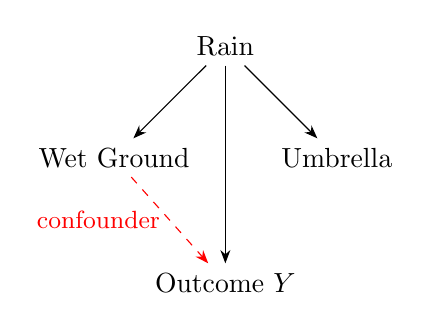
\begin{tikzpicture}[node distance=2cm]
\node (rain) {Rain};
\node (ground) [below left of=rain] {Wet Ground};
\node (umbrella) [below right of=rain] {Umbrella};
\node (outcome) [below of=rain, yshift=-1cm] {Outcome $Y$};

\draw[-{Stealth}] (rain) -- (ground);
\draw[-{Stealth}] (rain) -- (umbrella);
\draw[-{Stealth}] (rain) -- (outcome);
\draw[-{Stealth},dashed,red] (ground) -- (outcome) node[midway,left] {\small confounder};
\end{tikzpicture}
\end{center}

\begin{itemize}    \item $f_{\text{pred}}$: Uses ``Wet Ground'' as a predictor (valid correlation)
    \item $f_{\text{cause}}$: Identifies ``Rain'' as the causal mechanism
\end{itemize}
\end{example}

\subsection{The Causal-Predictive Conflict}

\begin{theorem}[Causal Divergence]
\label{thm:causal}
The predictive and causal objectives are generically non-aligned:
\begin{equation}
\boxed{\Dcausal = |f_{\text{pred}} - f_{\text{cause}}| > 0}
\end{equation}
whenever confounders are present in the feature set.
\end{theorem}

\begin{proof}
Let $X = \{X_{\text{causal}}, X_{\text{confound}}\}$ partition features into causal and confounding.

The predictive objective:
\begin{equation}
f_{\text{pred}} = \argmax_f P(Y | X_{\text{causal}}, X_{\text{confound}})
\end{equation}
utilizes both causal and confounding signals.

The causal objective:
\begin{equation}
f_{\text{cause}} = \argmax_f P(Y | \text{do}(X_{\text{causal}}))
\end{equation}
uses only interventional effects, excluding confounders.

Since $P(Y | X) \neq P(Y | \text{do}(X))$ in the presence of confounding:
\begin{equation}
f_{\text{pred}} \neq f_{\text{cause}} \implies \Dcausal > 0
\end{equation}
\end{proof}

\begin{figure}[ht]
\centering

\includegraphics[width=0.85\textwidth]{../figures/causal_divergence.png}
\caption{\textbf{Causal Divergence.} The conflict between predictive path $f_{\text{pred}}$ (using all correlations including confounders) and causal path $f_{\text{cause}}$ (identifying true mechanisms). The divergence $\Dcausal = |f_{\text{pred}} - f_{\text{cause}}|$ quantifies the epistemological gap.}
\label{fig:causal_divergence}
\end{figure}

\begin{corollary}[Interpretation Invalidity]
Interpreting $f_{\text{pred}}$ as if it were $f_{\text{cause}}$ leads to:
\begin{enumerate}    \item Spurious feature attributions (confounders appear important)
    \item Failed interventions (acting on ``Wet Ground'' does not produce ``Rain'')
    \item Vulnerability to distribution shift (confounding structure may change)
\end{enumerate}
\end{corollary}

%==============================================================================
\section{Synthesis: The Interpretation Lagrangian}
\label{sec:lagrangian}
%==============================================================================

We now synthesize the preceding derivations into a unified variational framework.

\begin{definition}[Interpretation Lagrangian]
The \textbf{Interpretation Lagrangian} is:
\begin{equation}
\boxed{\mathcal{L}_{\text{interp}} = \Dcausal + \lambda \Complex(f)}
\end{equation}
where:
\begin{itemize}    \item $\Dcausal = |f_{\text{pred}} - f_{\text{cause}}|$ is the causal divergence
    \item $\Complex(f)$ is the model complexity
    \item $\lambda > 0$ is a Lagrange multiplier (regularization coefficient)
\end{itemize}
\end{definition}

The Lagrangian captures the fundamental tension in IML:

\begin{proposition}[Trade-off Structure]
Minimizing $\mathcal{L}_{\text{interp}}$ requires balancing:
\begin{enumerate}    \item \textbf{Causal fidelity}: Minimize $\Dcausal$ (align prediction with causation)
    \item \textbf{Simplicity}: Minimize $\Complex(f)$ (maintain interpretability)
\end{enumerate}
\end{proposition}

\begin{theorem}[Optimal Interpretation]
The optimal interpretable model $f^*$ satisfies:
\begin{equation}
f^* = \argmin_{f \in \mathcal{H}} \left[ \Dcausal(f) + \lambda \Complex(f) \right]
\end{equation}
subject to constraints:
\begin{equation}
\begin{aligned}
&\text{Predictive constraint:} && P(Y|X; f) \geq P_{\min} \\
&\text{Manifold constraint:} && \text{supp}(f) \subseteq \Manifold \\
&\text{Uncertainty constraint:} && \Var(\Ocomp(f)) < \sigma^2_{\max}
\end{aligned}
\end{equation}
\end{theorem}

\subsection{Extended Lagrangian}

Incorporating the topological violations from Section~\ref{sec:topological}:

\begin{definition}[Extended Interpretation Lagrangian]
\begin{equation}
\mathcal{L}_{\text{ext}} = \Dcausal + \lambda_1 \Complex(f) + \lambda_2 \cdot \mathbb{1}[x' \notin \Manifold] + \lambda_3 \cdot \sigma^2_E
\end{equation}
where:
\begin{itemize}    \item $\lambda_2 \cdot \mathbb{1}[x' \notin \Manifold]$: Extrapolation penalty
    \item $\lambda_3 \cdot \sigma^2_E$: Uncertainty penalty
\end{itemize}
\end{definition}

\begin{remark}[Variational Principle]
The Interpretation Lagrangian defines a variational principle: the ``best'' interpretation minimizes causal divergence while respecting complexity constraints and avoiding topological violations.
\end{remark}

%==============================================================================
\section{The Complete Interpretability System}
\label{sec:complete}
%==============================================================================

We now present the complete formal specification of $\IML$.

\noindent\fbox{\parbox{\textwidth-2\fboxsep-2\fboxrule}{%
\textbf{The Interpretability System $\IML$}\\[0.5em]
\begin{equation}
\IML = \langle \mathcal{H}, \mathcal{O}, \mathcal{M}, \Delta \rangle
\end{equation}

\textbf{Hypothesis Space:}
\begin{equation}
\mathcal{H} = \Hstat \cup \Hml, \quad \Hstat \cap \Hml \to \emptyset \text{ as } \Complex \to \infty
\end{equation}

\textbf{Interpretation Operators:}
\begin{equation}
\mathcal{O} = \{\Ocomp, \Osens, \Osurr\}
\end{equation}
\begin{align}
\Ocomp(f) &= \theta & &\text{(decomposable } f \text{ only)} \\
\Osens(f,x) &= \nabla_x f(x) & &\text{(model-agnostic)} \\
\Osurr(f,x_0) &= g \in \Hstat & &\text{(local approximation)}
\end{align}

\textbf{Method Taxonomy:}
\begin{equation}
\mathcal{M} = \{\text{Component Analysis}, \text{Sensitivity Analysis}, \text{Surrogate Models}\}
\end{equation}

\textbf{Error Metric:}
\begin{equation}
\Delta = \{\Dcausal, \sigma^2_E, P(x' \notin \Manifold)\}
\end{equation}
}}

%==============================================================================
\section{Concluding Remarks}
%==============================================================================

This technical note has established a rigorous mathematical framework for interpretable machine learning, formalizing the epistemological structure through the Interpretability System tuple $\IML = \langle \mathcal{H}, \mathcal{O}, \mathcal{M}, \Delta \rangle$.

The key contributions are:

\begin{enumerate}
    \item \textbf{Evolutionary Divergence}: Formalization of the phase transition between statistical ($\Hstat$) and ML ($\Hml$) regimes, with the opacity theorem (Theorem~\ref{thm:opacity}) establishing the fundamental complexity-interpretability trade-off.

    \item \textbf{Operator Taxonomy}: Precise definitions of interpretation operators $\{\Ocomp, \Osens, \Osurr\}$ with explicit applicability conditions.

    \item \textbf{Topological Violations}: Proof of the extrapolation artifact (Theorem~\ref{thm:extrapolation}) and formalization of the uncertainty gap, establishing fundamental limits of perturbation-based interpretation.

    \item \textbf{Causal Divergence}: Formal demonstration that predictive and causal objectives are generically misaligned (Theorem~\ref{thm:causal}), with divergence metric $\Dcausal$.

    \item \textbf{Interpretation Lagrangian}: Synthesis of all components into the variational principle $\mathcal{L} = \Dcausal + \lambda \Complex(f)$, providing a unified framework for analyzing interpretation quality.
\end{enumerate}

This formalism provides a mathematical language for rigorously analyzing the epistemological limits of model interpretation, highlighting that \textit{interpretability is not a binary property but a constrained optimization over multiple competing objectives}.

\vspace{2em}
\hrule
\vspace{0.5em}
\begin{center}
\textit{Generated using K-Dense Web (\href{https://k-dense.ai}{k-dense.ai})}
\end{center}

%==============================================================================
% Bibliography
%==============================================================================
\bibliographystyle{plainnat}
\begin{thebibliography}{10}

\bibitem{molnar2020interpretable}
Molnar, C., Casalicchio, G., and Bischl, B. (2020).
\textit{Interpretable Machine Learning -- A Brief History, State-of-the-Art and Challenges}.
In: ECML PKDD 2020 Workshops. Communications in Computer and Information Science, vol 1323. Springer.

\bibitem{ribeiro2016lime}
Ribeiro, M.T., Singh, S., and Guestrin, C. (2016).
``Why Should I Trust You?'': Explaining the Predictions of Any Classifier.
In: \textit{Proceedings of the 22nd ACM SIGKDD International Conference on Knowledge Discovery and Data Mining}, pp. 1135--1144.

\bibitem{shapley1953value}
Shapley, L.S. (1953).
A Value for n-Person Games.
\textit{Contributions to the Theory of Games}, 2(28), 307--317.

\bibitem{breiman2001random}
Breiman, L. (2001).
Random Forests.
\textit{Machine Learning}, 45(1), 5--32.

\bibitem{pearl2009causality}
Pearl, J. (2009).
\textit{Causality: Models, Reasoning, and Inference}.
Cambridge University Press.

\end{thebibliography}

\end{document}
